\chapter{Evaluation}
\label{chap:eva}
\section{Setup}
The CLONALG algorithm will be applied to a set of 17 different TSP problems taken from the TSP library TSPLIB95 \footcite[https://www.iwr.uni-heidelberg.de/groups/comopt/software/TSPLIB95/]{tsplib}. The number after the name of the TSP is the amount of nodes and therefore indicates the difficulty of the TSP. The implementation follows the specification in \cite{DEC02} and is provided by the Optimization Algorithm Toolkit OAT \footcite[http://optalgtoolkit.sourceforge.net/]{oat}. All algorithms in the OAT are implemented in Java. The greedy search algorithm will be applied to the same set of problems, is provided by the author of the OAT and uses a nearest neighbour technique with mutation.\\\\ 
The stopping criteria for the algorithm will be no improvement after a set amount of evaluations. No improvement means the algorithm did not find a shorter route in it's current iteration compared to the last, this is also called stagnation. Every algorithm will run 100 times on one TSP, making it 1700 runs for all 17 TSP.
The criteria for the results are:
\begin{enumerate}
	\item 	Score
	\item 	Time in ms
	\item 	Evaluations	
	\item  	Percentage of optimal score
\end{enumerate}
Percentage of optimal score is the relative difference between the best possible route of the TSP and the result of the algorithm. The score is measured as the summarized Euclidean distance of the presented best tour. The algorithm will be run multiple times on one TSP, therefore the arithmetic mean of each criteria will be the end result. To compare results the mean average error (MAE) of the average score will be used. The MAE is composed of the difference between the score of both algorithms divided by the score of the compared algorithm. To compare the performance of algorithm A1 to A2 the MAE is calculated as $(A2-A1)/A1$. Positive MAE means better performance for A1. The significance of the difference is visible at the hundreds and tens digit, the thousands digit shows no significant difference. This was tested by running the complete test run twice on the same algorithm. Since the only difference between the single test runs was in the thousands digit it was not significant. The CLONALG algorithm will be applied to the problem set twice with different parameters. The adaptive algorithms will be applied only once because of the dynamic parameters.
The parameters to be altered are:
\begin{enumerate}
	\item 	Population size
	\item 	Clone factor
	\item 	Selection size
	\item 	Random replacements	
\end{enumerate}
The first set of parameters will be default parameters provided by the OAT as shown in table \ref{tuning}. The second set of parameters have been proposed by DeCastro \cite{DEC02} for solving TSP with a size of about 30 nodes.
The adaptive variant of the CLONALG algorithm will start with default values and adjust the parameters during runtime.
To measure the results, a modified version of the OAT will be used. The changes to the OAT consist of a slightly different set of TSP used in the domain and the addition of an adaptive CLONALG hybrid algorithm described in \ref{espc}. The used TSP are listed in table \ref{CLONALG_Avg}. The distances between nodes in the TSP problem are measured as Euclidean distance. The implemented CLONALG algorithm is based on the specifications in \cite{DEC02}. The adaptive variant expand the concept based on \cite{Garret04}.
Both algorithms will be applied 100 times on every TSP problem.\\\\
The hardware used consists of a i5-3320M dual core CPU with 2,60ghz each and 8gb of RAM, run on a Windows 10 operating system. All CPU and RAM usage shown in this thesis is after other processes, not related to the algorithm, are taken into account.
\subsection{Evolution Strategy Parameter Control}
\label{espc}
The adaptive CLONALG variation is based on \cite{Garret04} and uses a concept from the evolution strategy \cite{evolution}. The algorithm was able to eliminate all parameters except population size from the CLONALG algorithm. This thesis uses a variant where the selection size n is eliminated and is comparable to variant C1-C4 from \cite[p. 1054]{Garret04}. For this purpose the CLONALG implementation of the OAT is taken and modified based on the concepts in \cite{Garret04}. A strategy parameter adjusting selection size will be used. The strategy parameter itself will be adjusted by an evolution strategy constant of 1.3. This constant has been tested empirically and proven to be the most effective \cite{Garret04}. The adjustment will be randomized, the strategy parameter will be either multiplied or divided by the constant based on a 50\% chance. The strategy parameter itself will alter the selection size on each evaluation. However the difference to the original evolution strategy is that a parameter is indirectly adjusted through another parameter \cite{Garret04}. The algorithm used in this thesis generates the strategy parameter out of a gaussian random number, the result are the last selection size + the last strategy parameter * a random gaussian number. This is specific to the parameter generation in the OAT and is not necessary, the generation of the strategy parameter can be done in any other way suitable for the given application.  Naturally, the selection size still has to be initialized and can't be zero. As \cite{Garret04} proposed to start with a small number, the test runs in this thesis will start with a selection size of 1. Another difference to the orignial CLONALG is the absence of random replacements. The population will only be altered by the clones and their mutations. The changes made to the original pseudo code in chapter \ref{chap:ais} are shown in algorithm \ref{algo2}. This variant will be called CLONALG ESPC, standing for Evolution Strategy Parameter Control.\\\\
\begin{algorithm}[H]
	Set strategy paramater Sp\\
	Generate initial population C of A antibodies\\
	Oc=Calculate Fitness(C)\\
	\While{stopping criteria not met}{
		S= Select the n best antibodies from C\\
		P= Generate clones of the antibodies in S\\
		Mutate(P)\\
		C= Select the n best antibodies out of P\\
		C= C + New population A-n\\
		Nc= Calculate Fitness(C)\\
		If Nc has better fitness than Oc then\\
		n= Sp * 1.3 OR n= Sp/1.3\\
		else\\
		n=n\\
		end if\\
		Oc=Nc\\
	}
	\caption{CLONALG variant with dynamic selection size}
	\label{algo2}
\end{algorithm}
\section{Results: Improvement Limitation}
\subsection{CLONALG untuned}
The algorithms are run 100 times on every TSP. The stopping criteria are defined as no improvements after 10000 iterations of the algorithm. This number is chosen to give the algorithm enough time without restricting it to a specific amount of seconds. The CPU usage spiked around 58\% with an average around 30\% for all algorithms. This is because the more costly operations like sorting, selection, cloning and mutation will be done in exactly the same way in all algorithms.
The parameters for the original CLONALG are shown in Table \ref{tuning}.\\
The parameter C stands for the initial population, n for the selection size for cloning, B for cloning factor (how many clones of the chosen n will be made) and d for random replacements to keep the new population partially randomized. \cite{DEC02} proposed tuning the default parameters for more efficiency in solving TSP. The replacement value d should always be between 5-20\% of the population since higher ratios tend to randomize too much while lower ratios still produce good but less reliable and efficient results \cite{DEC02}.\\\\
\begin{table}[H]
	\begin{tabular}{|c|c|c|c|c|}
		\hline
		& C   & n   & B   & d  \\ \hline
		Default & 50  & 50  & 0.1 & 5  \\ \hline
		Tuned   & 300 & 150 & 2.0 & 60 \\ \hline
	\end{tabular}
	\caption{Tuning parameters}
	\label{tuning}
\end{table} 
Comparing the performance of the untuned CLONALG to the greedy algorithm shows that the CLONALG algorithm on average performs worse than the greedy search algorithm (figure \ref{CLONALG_Avg}). However the CLONALG was able to find the best solution to the TSP ulysses22 with a MAE of 0.117, while the greedy search algorithm could not as shown in table \ref{tab:clonalg_untuned}.In addition the overall time for solving all problems was also shorter for the CLONALG. The number of evaluations is most of the time smaller for the CLONALG showing that stagnation started earlier. The average MAE for all TSP compared to the greedy algorithm is -0.524. The average MAE for all TSP calculated on the best instead of the average score is in the same range with with a result of -0.546. The mean average error of -0.009 is not significant for the TSP berlin52, highlighting that CLONALG performs equaly good or better on small TSP under 50 nodes, but is less efficient at more difficult TSP compared to the greedy algorithm.
\begin{figure}[H]
	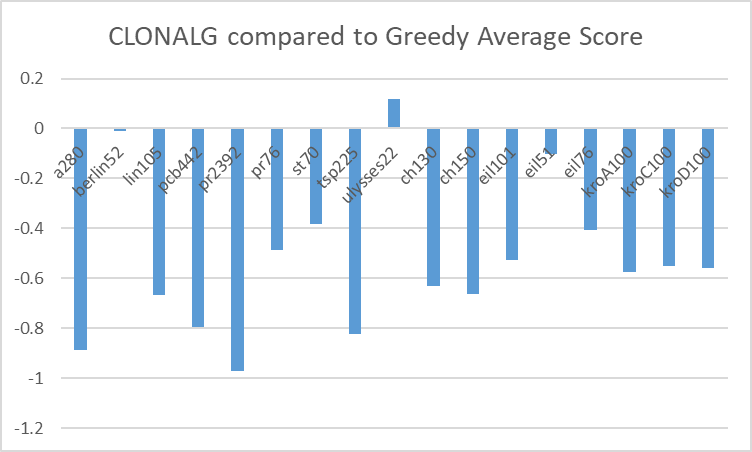
\includegraphics[height=8cm, width=13cm]{Images/CLONALG_Fig_Avg2.png}
	\caption{MAE on Average Score for CLONALG compared to greedy}
	\label{CLONALG_Avg}
\end{figure}
\begin{table}[H]
	\begin{tabular}{|l|l|l|p{2cm}|p{2.5cm}|p{2cm}|}
		\hline
	TSP	& Avgerage Score & Best Score & Best Percentage &\textbf{ MAE compared to greedy} & Average Evaluations \\ \hline
		a280      & 26483.99       & 25581      & 891.896     & -0.885           & 38462.71            \\ \hline
		berlin52  & 11077.22       & 9369       & 24.224     & -0.009          & 132557.69           \\ \hline
		lin105    & 69431.08       & 62981      & 338.007     & -0.667           & 59348.99            \\ \hline
		pcb442    & 649513.41      & 631174     & 1143.007     & -0.796           & 38322.66            \\ \hline
		pr2392    & 14231642.92    & 14122859   & 3635.890     & -0.972           & 32506.49            \\ \hline
		pr76      & 299815.73      & 267781     & 147.581     & -0.487           & 73496.26            \\ \hline
		st70      & 1765.09        & 1510       & 123.704     & -0.383           & 82887.36            \\ \hline
		tsp225    & 31309.96       & 29905      & 663.662     & -0.822           & 41252.29            \\ \hline
		ulysses22 & 7273.04        & 6901       & 0               & 0.117            & 27588.51            \\ \hline
		ch130     & 31453          & 29391      & 381.031     & -0.631           & 46159.77            \\ \hline
		ch150     & 37883.24       & 36015      & 451.700     & -0.661           & 47285.45            \\ \hline
		eil101    & 2126.54        & 1954       & 210.652     & -0.525           & 56058.04            \\ \hline
		eil51     & 654.65         & 552        & 29.577     & -0.103           & 115597.85           \\ \hline
		eil76     & 1377.39        & 1194       & 121.933     & -0.408           & 67914.53            \\ \hline
		kroA100   & 96214.68       & 86675      & 307.269     & -0.573           & 60339.55            \\ \hline
		kroC100   & 94471.33       & 85368      & 311.432     & -0.550           & 60015.33            \\ \hline
		kroD100   & 93282          & 84305      & 295.910     & -0.558           & 57958.20            \\ \hline
	\end{tabular}
	\caption{CLONALG untuned performance}
	\label{tab:clonalg_untuned}
\end{table}
\subsection{CLONALG tuned}
Comparing the tuned algorithm to the original one shows that the tuned parameters are not suited for the tested TSP setup. The tuned CLONALG has a worse average score in solving all 17 TSP compared to the untuned CLONALG. An unexpected outcome is that the tuned algorithm performs better on larger TSP. The MAE on pr2392, the largest TSP in the setup, is only -0.014 whereas the MAE of ulysses22, the smallest TSP, is -0.305. The algorithm could not find the best solution for ulysses22. Compared to the untuned algorithm the average MAE for all TSP was -0.253. This is especially unexpected because the parameters where tuned by \cite{DEC02} for a 30 nodes TSP. In their tests, the tuned algorithm behaved better on this TSP than the untuned one. The results show that the chosen parameters do not work well if the stopping criteria are 10000 evaluations without improvement.
\begin{table}[H]
	\begin{tabular}{|l|l|l|l|p{2.5cm}|p{2cm}|}
		\hline
		TSP       & Avgerage Score & Best Score & Best Percentage    &\textbf{ MAE compared to CLONALG} & Average Evaluations  \\ \hline
		a280      & 29313.63    & 27910     & 982.202  & -0.097                                                     & 12173.27 \\ \hline
		berlin52  & 22284.75    & 20861     & 176.598 & -0.501                                                    & 13140.05 \\ \hline
		lin105    & 95696.8     & 89181     & 520.217 & -0.274                                                    & 12437.46 \\ \hline
		pcb442    & 695194.14   & 680524    & 1240.195 & -0.066                                                    & 12179.71 \\ \hline
		pr2392    & 14434730.31 & 14288477  & 3679.700 & -0.014                                                   & 11541.92 \\ \hline
		pr76      & 445633.5    & 418899    & 287.299 & -0.327                                                    & 12718.28 \\ \hline
		st70      & 2826.17     & 2672      & 295.852 & -0.375                                                    & 12650.36 \\ \hline
		tsp225    & 35353.65    & 32603     & 732.559 & -0.114                                                    & 12485.88 \\ \hline
		ulysses22 & 10459.55    & 9389      & 36.0527 & -0.305                                                    & 13776.71 \\ \hline
		ch130     & 38766.46    & 36521     & 497.725 & -0.189                                                    & 13543.46 \\ \hline
		ch150     & 45610.23    & 43708     & 569.547 & -0.169                                                    & 12907.27 \\ \hline
		eil101    & 2773.71     & 2685      & 326.868 & -0.233                                                    & 13245.55 \\ \hline
		eil51     & 1240.14     & 1170      & 174.648 & -0.472                                                    & 13879.30 \\ \hline
		eil76     & 1993        & 1806      & 235.688 & -0.309                                                    & 13296.35 \\ \hline
		kroA100   & 134148.49   & 125461    & 489.517 & -0.283                                                    & 13492.89 \\ \hline
		kroC100   & 132863.13   & 126691    & 510.588 & -0.289                                                    & 13778.59 \\ \hline
		kroD100   & 129082.57   & 124611    & 485.193 & -0.277                                                    & 14173.76 \\ \hline
	\end{tabular}
	\caption{CLONALG tuned performance}
	\label{tab:clonalg_tuned}
\end{table}
\subsection{CLONALG ESPC}
The variant with an adaptive selection size shows only an insignificantly worse performance with an average MAE of -0.009 for all TSP compared to the tuned CLONALG. An interesting behaviour is seen in the average MAE for all TSP calculated on the best score with 0.039. This value shows that the adaptive CLONALG is better suited to finding the shorter route, but will also produce some worse solutions in the long run. The MAE on the best score was significantly better on eil101, kroA100 and kroD100, the bigger TSP in this setup. These results highlight that an adaptive selection size altered with the evolution strategy and combined with no random replacements can be beneficial to finding the shorter route. On average the CLONALG ESPC needed less evaluations to terminate, the stagnation started earlier. The overall runtime was nearly identical for the original CLONALG and the ESPC, with close to 19 minutes for a complete test run on all 17 TSP. Comparing the ESPC to the greedy algorithm still shows a worse performance of the ESPC, both on average score and in the majority of the best scores. The ESPC found the shorter route on berlin52 with a MAE of 0.022 and the best route on ulysses22 with a MAE of 0.011. The modification enhanced the ability of the algorithm in solving smaller TSP compared to the greedy algorithm, but did not have a measurable impact on its performance on greater TSP (figure \ref{ESCP_greedy}).\\
\begin{figure}[h]
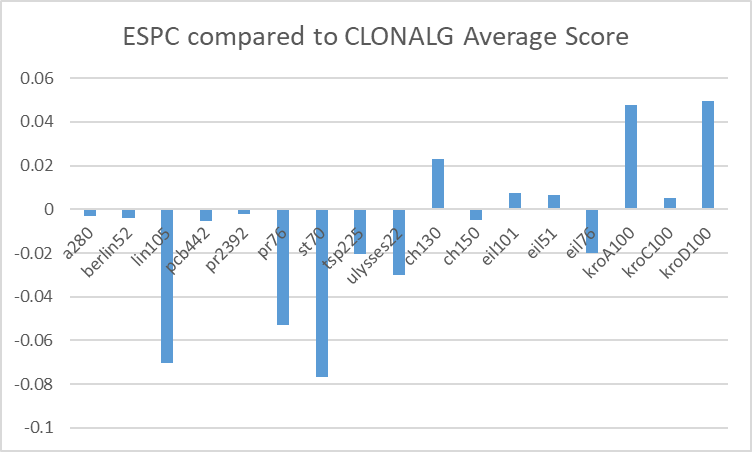
\includegraphics[height=8cm,width=13cm]{Images/ESPC_Fig_Avg2.png}
\caption{MAE on Average Score for ESPC compared to CLONALG}
\label{ESCP_AVG}
\end{figure}
\begin{figure}[H]
	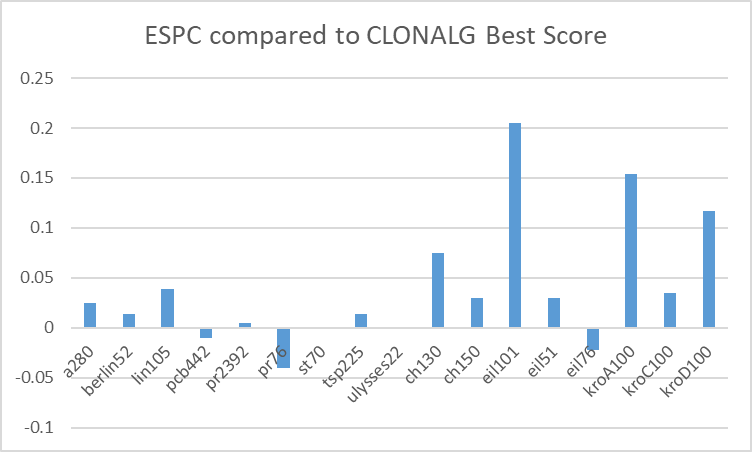
\includegraphics[height=8cm,width=13cm]{Images/ESPC_Fig_Best2.png}
	\caption{MAE on Best Score for ESPC compared to CLONALG}
	\label{ESCP_Best}
\end{figure}
\begin{figure}[H]
	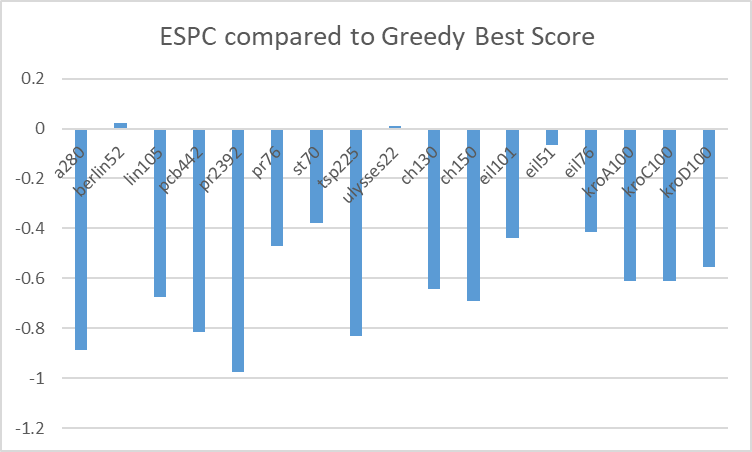
\includegraphics[height=8cm,width=13cm]{Images/ESPC_Fig_Greedy2.png}
	\caption{MAE on Best Score for ESPC compared to greedy}
	\label{ESCP_greedy}
\end{figure}
\begin{table}[H]
	\begin{tabular}{|l|p{2cm}|p{1.6cm}|p{2.2cm}|p{2.4cm}|p{2.4cm}|p{1.7cm}|}
		\hline
		TSP       & Average Score & Best Score & Best Percentage &\textbf{ MAE compared to CLONALG} & MAE on Best Score compared to CLONALG & Average Evalutions \\ \hline
		a280      & 26559.75      & 24949      & 867.390     & -0.003            & 0.025       & 34025.59           \\ \hline
		berlin52  & 11120.65      & 9241       & 22.527     & -0.004            & 0.014       & 173022.70          \\ \hline
		lin105    & 74683.73      & 60638      & 321.712     & -0.070            & 0.039       & 48963.38           \\ \hline
		pcb442    & 652981.26     & 637838     & 1156.131     & -0.005            & -0.010      & 35590.02           \\ \hline
		pr2392    & 14259316.88   & 14060841   & 3619.484     & -0.002            & 0.004       & 31152.73           \\ \hline
		pr76      & 316531.58     & 278997     & 157.951     & -0.052            & -0.040      & 64605.41           \\ \hline
		st70      & 1912.1        & 1511       & 123.852     & -0.077            & -0.001      & 68687.03           \\ \hline
		tsp225    & 31963.99      & 29509      & 653.550     & -0.020            & 0.013       & 36970.86           \\ \hline
		ulysses22 & 7499.74       & 6901       & 0               & -0.030            & 0                 & 27280.05           \\ \hline
		ch130     & 30748.35      & 27332      & 347.332     & 0.023             & 0.075       & 45024.26           \\ \hline
		ch150     & 38069.35      & 34981      & 435.861     & -0.005             & 0.030       & 40273.29           \\ \hline
		eil101    & 2111.16       & 1622       & 157.870     & 0.007             & 0.205       & 53395.42           \\ \hline
		eil51     & 650.27        & 536        & 25.822     & 0.007             & 0.030       & 118097.23          \\ \hline
		eil76     & 1405.74       & 1221       & 126.952     & -0.020            & -0.022      & 62993.43           \\ \hline
		kroA100   & 91818.4       & 75100      & 252.880     & 0.048             & 0.154        & 62252.60           \\ \hline
		kroC100   & 94006.78      & 82471      & 297.470     & 0.005             & 0.035       & 57812.68           \\ \hline
		kroD100   & 88897.32      & 75500      & 254.560     & 0.049             & 0.117       & 58883.91           \\ \hline
	\end{tabular}
	\caption{ESPC performance}
	\label{tab:espc}
\end{table}
When looking at the average percentage the algorithms deviate from the best solution, the greedy algorithm outclasses the CLONALG variants. The average percentage for the greedy is 63.7, the untuned CLONALG achieves 566.6, the tuned CLONALG 693.1 and the ESPC 570.2. These values on their own are not suited to judge the performance of the algorithm because of the wide range in difficulty of the TSP, but the difference compared to the greedy algorithm is very high.\\ The greedy algorithm needed about 52 minutes to complete the whole test run, while the CLONALG variants needed about 19 minutes.
\section{Results: Time Limitation}
To test if a fixed amount of runtime yields different results than the no improvements criteria, the algorithms will be applied to another test run. In this run every algorithm runs once on every TSP. The stopping criteria is 25 seconds.\\
The CLONALG has an average MAE of -0.328 for all TSP compared to the greedy algorithm. This is better than with the criteria set to 10000 iterations without improvement, where this MAE was -0.546. This time the CLONALG achieved a better score on the TSP berlin52, ulysses22, st70, eil51 and eil76 (figure\ref{CLONALG_Time}). The performance of the CLONALG was better with this stopping criteria.
\begin{figure}[H]
	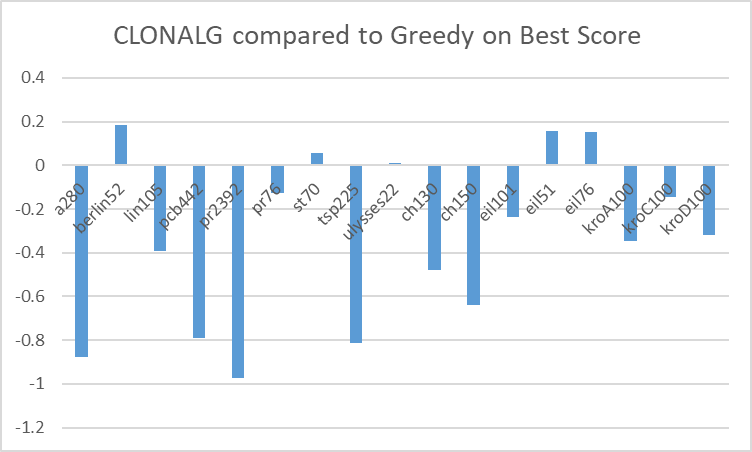
\includegraphics[height=8cm,width=13cm]{Images/CLONALG_Time2.png}
	\caption{MAE on Best Score for CLONALG compared to greedy with the 25 seconds stopping criteria}
	\label{CLONALG_Time}
\end{figure}
The tuned CLONALG algorithm still performs worse than the untuned, but can achieve a better score for ulysses22, berlin52 and eil51 than the greedy algorithm. It was also able to find a better route for ulysses22 compared to the tuned and the ESPC variant, which was not possible in the previous evaluation.\\
The ESPC has an average MAE of 0.110 for all TSP compared to the CLONALG and achieves a better score on all TSP except berlin52, st70, eil51, and eil76 (table \ref{ESPC_Time})). The ESPC also shows a better performance when running for 25 seconds compared to the no improvements criteria.
\begin{figure}[H]
	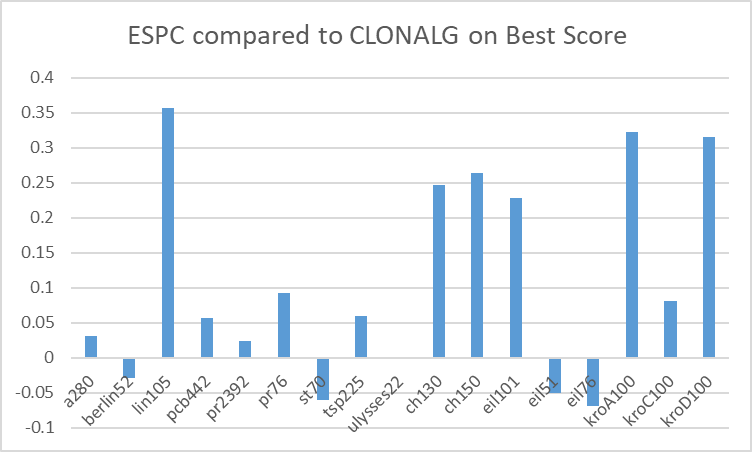
\includegraphics[height=8cm,width=13cm]{Images/ESPC_Time2.png}
	\caption{MAE on Best Score for ESPC compared to CLONALG with the 25 seconds stopping criteria}
	\label{ESPC_Time}
\end{figure}
The average MAE compared to the greedy algorithm is -0.270, which is better than the previous evaluation of -0.530. The ESPC scored better on the TSP berlin52, ulysses22, eil51 and eil76. These are the same TSP where the ESPC had a worse score than the CLONALG.
\begin{figure}[H]
	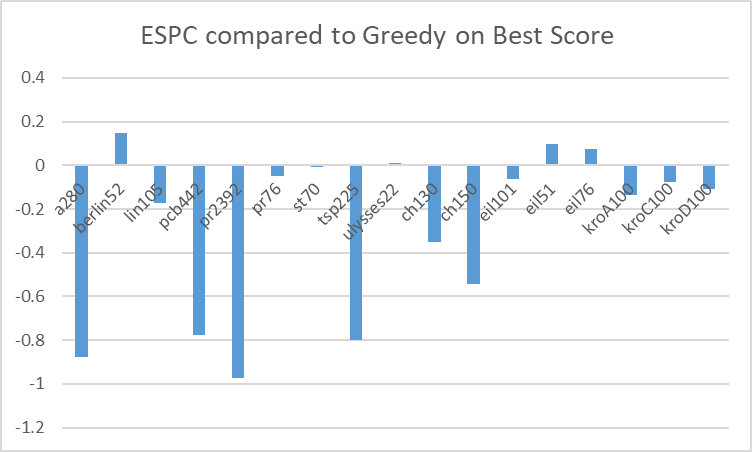
\includegraphics[height=8cm,width=13cm]{Images/ESPC_Greedy_Time2.png}
	\caption{MAE on Best Score for ESPC compared to greedy with the 25 seconds stopping criteria}
	\label{ESPC_greedy_TIME}
\end{figure}
\newpage
The average deviation percentage from the best score became better for all algorithms, but to a different degree. The greedy algorithm now deviates 54.2, the untuned CLONALG 447.2, the tuned CLONALG 529.6 and the ESPC 410.9 percent. These values highlight that the CLONALG variants profit more from a longer runtime in solving the TSP than the greedy algorithm. The deviation for the CLONALG variants improved more than 100 percent, but still remained very high compared to the greedy algorithm (table \ref{avgDeviation}). This is best seen on the largest TSP pr2392, where all clonal algorithms had a deviation from optimal score of more than 3000 percent. The greedy algorithm shows an exceptional performance on pr2392, with only over 1 percent deviation from optimal score, however, this TSP is highly structured and organized (figure \ref{pr2392}). The nearest-neighbour technique of this algorithm is suited for solving this TSP, but is less efficient at less structured and more random TSP. The clonal algorithms do not benefit from any kind of order, symmetry or structure in the TSP, but they are also not negatively affected by the lack thereof. 
\begin{figure}[H]
	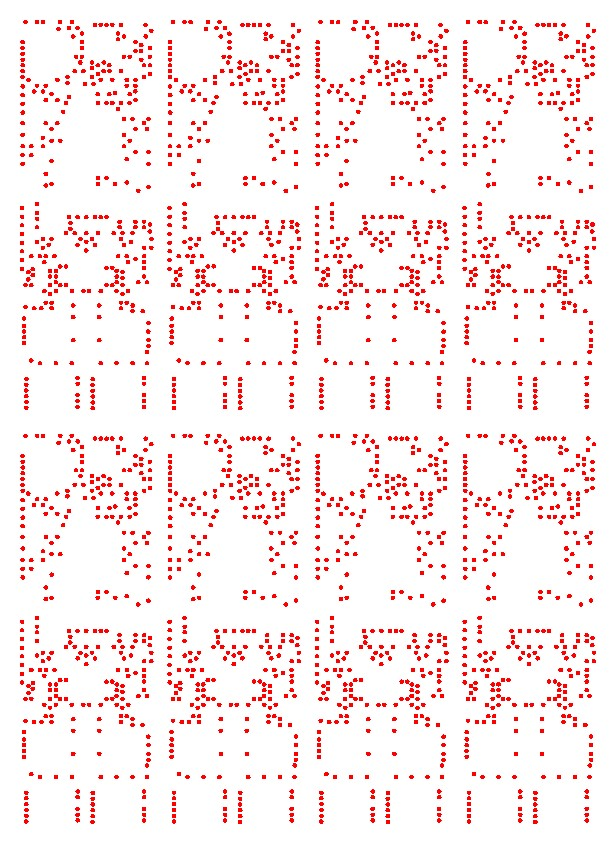
\includegraphics[width=10cm, height=15cm]{Images/pr2392.jpg}
	\caption{pr2392 the largest TSP in the setup (source: OAT)}
	\label{pr2392}
\end{figure}
\begin{table}[H]
	\begin{tabular}{|l|l|l|}
		\hline
		\textbf{\begin{tabular}[c]{@{}l@{}}Average deviation\\ percentage from\\ optimal score\end{tabular}} & \textbf{\begin{tabular}[c]{@{}l@{}}10000 iterations\\ without improvement\\ stopping criteria\end{tabular}} & \textbf{\begin{tabular}[c]{@{}l@{}}25 seconds\\ stopping criteria\end{tabular}} \\ \hline
		\textbf{Greedy}                                                                         & 63.7                                                                                                        & 54.2                                                                            \\ \hline
		\textbf{CLONALG tuned}                                                                  & 693.1                                                                                                       & 592.6                                                                           \\ \hline
		\textbf{CLONALG untuned}                                                                & 566.6                                                                                                       & 447.2                                                                           \\ \hline
		\textbf{ESPC}                                                                           & 570.2                                                                                                       & 410.9                                                                           \\ \hline
	\end{tabular}
	\caption{Average deviation from optimal score}
	\label{avgDeviation}
\end{table}
 
